{\textbf{1. 复杂度总结}}{}

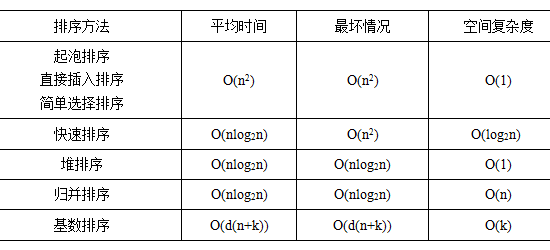
\includegraphics[width=3.70833in,height=1.68750in]{png-jpeg-pics/0DF3E739B360E9D3730BB2F37C5685AC.png}

{\textbf{2. 稳定性}}

{不稳定的排序方法有:快速排序、希尔排序、简单选择排序、堆排序。}{其余排序方法都是稳定的。}

{\textbf{3. 一趟排序确定一个元素位置的排序方法}}

{凡是每趟产生的有序区为全局有序区的排序方法,则每一趟排序结束时都至少能够确定一个元素的最终位置,这样的排序方法有简单选择排序、堆排序和快速排序。快速排序尽管不是每趟都产生有序区,但它将基准元素放在最终位置上。}

{\textbf{4. 元素比较次数与原始序列无关的排序方法}}

{简单选择排序和折半插入排序。}
